\subsection{Parallel Implementation of Iterative Methods}
\label{section:parallel}
The iterative methods are ideal for their low memory requirements, and this becomes extremely important as the simulations in many fields of study have moved towards three-dimensional models. Another appealing part of iterative methods is that they are far easier to implement in parallel than sparse direct methods because they only require a small set of computational kernels. However, iterative methods are usually slower than direct methods, especially for smaller problems, requiring suitable preconditioning techniques for accelerated convergence. The parallel aspect of preconditioners also becomes very important naturally.

This subsection gives a short overview of various parallel architectures as well as different types of operations in iterative methods that can be parallelized.

% \subsubsection{Different Parallel Architectures}
There are currently three leading architectures of parallel models around which modern parallel computers are designed. These are
\begin{itemize}
    \item The shared-memory model
    \item Single-instruction-multiple-data (SIMD)
    \item The distributed memory message passing model
\end{itemize}

\subsubsection{Shared memory computers}
A shared memory computer has processors connected to a large global memory, and the address space is the same for all processors. Data stored in a large global memory is readily accessible to any processor. Traditionally, there are two possible implementations of shared memory machines: 
\begin{itemize}
    \item bus-based architectures
    \item switch-based architectures
\end{itemize}

\begin{figure}[h!]
    \centering
    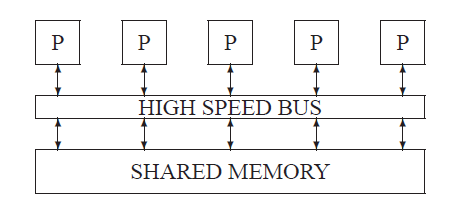
\includegraphics[width=\linewidth]{figures/bus-based-shared-memory.png}
    \caption{A bus-based shared memory computer \citep{doi:10.1137/1.9780898718003}}
    \label{fig:bus-shared}
\end{figure}

\begin{figure}[h!]
    \centering
    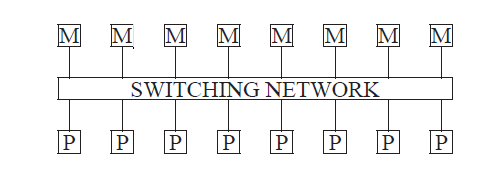
\includegraphics[width=\linewidth]{figures/switch-based-shared-memory.png}
    \caption{A switch-based shared memory machine \citep{doi:10.1137/1.9780898718003}}
    \label{fig:switch-shared}
\end{figure}

These two architectures are illustrated in \autoref{fig:bus-shared} and \autoref{fig:switch-shared}. So far, the bus-based model has been used more often. Buses are the backbone for communication between the different units of most computers, and usually have higher bandwidth for data I/O. The main reason why the bus-based model is more common is that the hardware involved in such implementation is simpler \citep{adeli1987parallel}. However, memory conflicts as well as the necessity to maintain data coherence can lead to worse performance. Moreover, shared memory computers can not take advantage of data locality in problems such as solving PDEs. Some machines can even have logically shared but physically distributed memory.
Modern HPC CPUs have ring meshes and Non-Uniform Memory Access (NUMA) to address challenges of scalability and communication \citep{569606,10.1145/1854273.1854350}.

\subsubsection{Distributed Memory Architectures}
The \textit{distributed memory} model can refer to distributed memory SIMD architecture or distributed memory with \textit{memory passing} interface. A typical distributed memory system consists of a large number of identical processors and each processor has its own memory. These processors are interconnected in a regular topology. This can be shown with \autoref{fig:distributed-memory}. In these diagrams, each processor unit can be viewed as a complete processor with its one memory, CPU, I/O subsystems, control unit, etc. These processors are linked to a number of ``neighboring'' processors. In the ``message passing'' model, no global synchronizations are performed of the parallel tasks. Instead, computations are \textit{data driven} because each processor performs a given task only when the operands it requires become available. The programmer needs to explicitly instruct data exchanges between different processors.

\begin{figure}
    \centering
    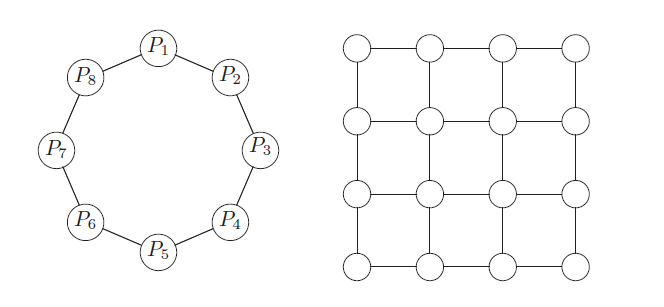
\includegraphics[width=\linewidth]{figures/distributed-memory.png}
    \caption{An eight-processing ring (left) and 4 $\times$ 4 multiprocessor mesh (right) \citep{doi:10.1137/1.9780898718003}}
    \label{fig:distributed-memory}
\end{figure}



In the SIMD model, a different approach is used. A host processor stores the program and each slave processor holds different data. The host broadcasts instructions to each processor to execute them simultaneously. One advantage of this approach is that there is no need for large memories in each node to store the main program since the same instructions are broadcast to each processor.

Unlike the shared-memory model, distributed memory computers can easily exploit the data locality of data to reduce communication costs. Modern GPUs are designed with the SIMD model (more accelerately Single-instruction-multiple-threads, SIMT) \citep{owens2008gpu}, and clusters with multiple CPUs are connected using a message passing interface (MPI) \citep{barker2015message}.


\subsection{Key Operations in Parallel Implementation}
\subsubsection{Types of Operations}

We use the preconditioned Conjugate Gradient (PCG) to demonstrate the typical operations involved that can be parallelized. The PCG algorithm consists of the following types of operations:
\begin{itemize}
    \item Preconditioner setup
    \item Matrix-vector multiplications
    \item Vector update
    \item Dot Product
    \item Preconditioning operations
\end{itemize}

Matrix-vector multiplications, vector updates, and dot products are common operations in so-called Basic Linear Algebra Subprograms (BLAS) that can be easily parallelized and have been well studied and implemented for dense matrices\citep{10.1145/77626.79170,chtchelkanova1997parallel,freeman1992parallel}. In terms of the computational costs, the vector update and dot product are much lower compared to the matrix-vector multiplication, which can still be carried out very quickly on the latest GPUs. The tricky part or the bottleneck for both memory and the runtime lies in the first step of preconditioner setup and the last step of preconditioning operations. We will discuss these two key operations in the next subsection. For now, let's focus on the matrix-vector multiplication that has much higher computational costs than the vector update and the dot product.

\subsubsection{Sparse Matrix-Vector Products}
The linear system coming from the discretization in the finite difference method is often sparse, which allows us to store them efficiently and use Sparse Matrix-Vector Products (SpMVs) for efficient computation. Different formats for storing sparse matrices can be found in \citep{doi:10.1137/1.9780898718003}. Compressed Sparse Row (CSR) sparse matrix format is one of the earliest sparse formats developed. It is ideal for parallelization since the data from each row can be handled independently. The SpMV algorithm for CSR format as well as the demonstration of the storage scheme of the CSR format is shown in \autoref{fig:csr}

\begin{figure}[h!]
    \centering
    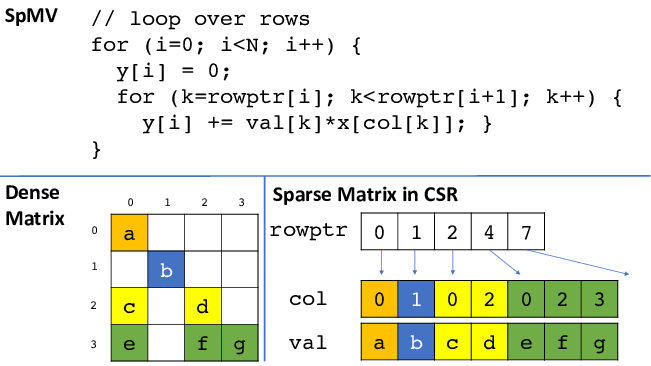
\includegraphics[width=\linewidth]{figures/Compressed-Sparse-Row-CSR-sparse-matrix-format-The-val-array-stores-the-nonzeros-by.png}
    \caption{The \texttt{val} array stores the nonzeros by packing each row in contiguous locations. The \texttt{rowptr} array points to the start of each row in the \texttt{val} array. The \texttt{col} array is parallel to \texttt{val} and maps each nonzero to the corresponding column.\citep{mohammadi2018sparse}}
    \label{fig:csr}
\end{figure}



A summary of different sparse matrix formats in the following table as well as a detailed performance comparison of these different formats can be found in \citep{stanimirovic2009performance}.
\begin{table}[h!]
\begin{tabular}{llll}
\toprule
Short & Name  & Short & Name            \\
\midrule
DNS        & Dense & Ell        & Ell-pack ItPack \\
BND           & Linpack Banded      &  DIA            & Diagonal                \\
COO           & Coordinate      & BSR           &  Block Sparse Row               \\
CSR           & Compressed Sparse Row      &    SSK        &    Symmetric Skyline             \\
CSC           &  Compressed Sparse column      & BSR           &  Nonsymmetric Skyline               \\
MSR           & Modified CSR       &    JAD        &    Jagged Diagonal             \\
    LIL       & Linked List      &            &                \\
\bottomrule
\end{tabular}
\caption{A summary of different sparse matrix formats and their short names}
\end{table}
There are also recent work on developing new sparse matrix formats for optimal performance for different use cases \citep{smailbegovic2005sparse,dongarraxz1994sparse} or implementing SpMV algorithms on parallel architectures \citep{bell2009,yan2014yaspmv,li2014performance}. Using the right sparse matrix formats and implementing them on suitable architectures can reduce the time spent on these SpMV calculations significantly, which makes iterative methods run faster. Another way to accelerate these iterative methods is to use the preconditioners that we mentioned before. A parallel implementation of these preconditioners becomes more challenging because of the complex arithmetic operations compared to the SpMV or other BLAS operations. We will focus on the parallel preconditioning technique in the next subsection.




\subsection{Parallel Preconditioning}

\subsubsection{Parallelism in Solving Linear Systems}
Each preconditioned step from the previous subsection requires the solution of a linear system of equations of the form $Mz = y$. We consider traditional preconditioners such as ILU or SOR or SSOR, in which a solution with $M$ is the result of solving triangular systems. Since these preconditioners are commonly used, it's important to explore their efficient parallel implementations for the iterative methods to be parallel. These preconditioners are mostly implemented on shared memory parameters. The distributed memory computers would use different strategies. These preconditioners require some sort of factorization, and the parallelism is done by sweeping through the lower triangular matrix or upper triangular matrix. Typical parallelism can be seen using a forward sweep. 

It's typical for solving a lower triangular system that the solution is overwritten onto the right-hand side. So there is only one array $u$ needed for both the solution and the right-hand side. The forward sweep for solving lower triangular systems with coefficients $A(i,j)$ and right-hand-side $b$ is defined as follows:
% \begin{algorithm}
% \caption{Sparse Forward Elimination}\label{alg:two}ß
%     \For{$i = 2 \dots n$}{
%         \For{ \text{all $j$ that $A(i,j)$ is nonzero}}{
%             $u(i)$ $\gets$ $u(i) - A(i,j) * u(j)$    \\
%         }
%     }
% \end{algorithm}
\begin{algorithm}
\caption{Sparse Forward Elimination}\label{alg:two}
\begin{algorithmic}[1]
    \For{$i \gets 2$ to $n$}
        \For{each $j$ such that $A(i,j) \neq 0$}
            \State $u(i) \gets u(i) - A(i,j) \times u(j)$
        \EndFor
    \EndFor
\end{algorithmic}
\end{algorithm}

Here $A(i,j)$ refers to the element in the sparse matrix. The different sparse matrix formats will have different implementations of locating this element, so the inner for loop will be implemented differently and the $A(i,j)$ will be replaced by different indexing code in different sparse matrix formats.

\subsubsection{Parallel preconditioners}
Several techniques can be for parallel implementations of the preconditioners. They can be summarized into three types of techniques.
The simplest approach is to use a Jacobi or block Jacobi approach. In this case, a Jacobi preconditioner may be consist of a diagonal or a block-diagonal of $A$
To improve the performance, these preconditioners can be accelerated by polynomial iterations. For example, the second level of preconditioning is called \textit{polynomial preconditioning}.
A different strategy is to enhance parallelism by using graph algorithms, such as graph-coloring techniques. The gist of this approach is that all unknowns associated with the same color can be determined simultaneously in the forward or backward sweeps.
The third strategy uses generalizations of ``partitioning'' techniques which can be also called ``domain decomposition'' approaches.
We will give a brief overview of these methods in this part.

Overlapping block-Jacobi preconditioning is a parallel preconditioner similar to the general block-Jacobi approach with overlapping blocks as shown in \autoref{fig:overlap-block-jacobi}. Enlarging a system of algebraic equations by including duplicate copies of several rows, leads to an efficient iterative scheme on a multiprocessor MIMD array \citep{WAIT1988325}. 
\begin{figure}[h!]
    \centering
    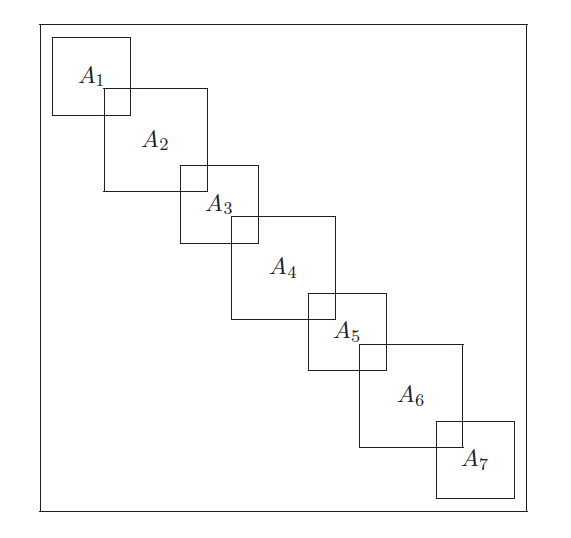
\includegraphics[width=\linewidth]{figures/block-jacobi.png}
    \caption{The block-Jacobi matrix with overlapping blocks \citep{doi:10.1137/1.9780898718003}}
    \label{fig:overlap-block-jacobi}
\end{figure}


Polynomial preconditioners are another family of parallel preconditioners. In polynomial preconditioners, the matrix $\boldsymbol{M}$ is defined by $\boldsymbol{M^{-1} = s(A)}$, where $\boldsymbol{s}$ is a polynomial, typically of low degree. Thus the original system can be preconditioned by 
\begin{equation}
    \boldsymbol{s(A)Au = s(A)f}
\end{equation}
Note that the $\boldsymbol{s(A)}$ and $\boldsymbol{A}$ commute, and as a result, the preconditioned matrix is the same for left or right preconditioning. In addition, the matrix $\boldsymbol{s(A)}$ or $\boldsymbol{As(A)}$ does not need to be formed explicitly in matrix form, which allows the use of matrix-free methods.
This approach was initially motivated by the good performance of matrix-vector operations on vector computers. It has now become more popular on iterative methods for GPU computing because of the similar SIMD architecture. 
There are several ways to construct polynomials in this method.
% The simplest polynomial $s$ is the polynomial of the Neumann series expansion
% \begin{equation}
%     I + N + N^2 + \cdots + N^s
% \end{equation}
% In which
% \begin{equation}
%     N = I - \omega A
% \end{equation}
% $\omega$ is called the scaling parameter. The series above comes from expanding the inverse of $\omega A$ using the splitting
% \begin{equation}
%     \omega A = I - (I - \omega A)
% \end{equation}
% This approach can be generalized using the splitting of the form
% \begin{equation}
%     \omega A = D - (D - \omega A)
% \end{equation}
% where $D$ can be a diagonal of A, or a block diagonal of A.
% Then
% \begin{align}
%     (\omega A)^{-1} &= [D(I - (I - \omega D^{-1}A))]^{-1} \nonumber \\
%     &= [I - (I - \omega D^{-1}A)]^{-1}D^{-1}
% \end{align}
% Thus, setting
% \begin{equation}
%     N = I - \omega D^{-1}A
% \end{equation}
% results in the approximate $s$-term expansion
% \begin{equation}
%     (\omega A)^{-1} \approx M^{-1} = [I + N + \cdots + N^s]D^{-1}
% \end{equation}
% Since $D^{-1}A = \omega^{-1}[I - N]$, note that

% \begin{align}
%     M^{-1}A & = [I + N + \cdots + N^s]D^{-1}A \nonumber \\
%     &= \frac{1}{\omega}[I + N + \cdots + N^2](I - N) \nonumber \\
%     &= \frac{1}{\omega}(I - N^{s+1})
% \end{align}


% The matrix operation with the preconditioned matrix can be difficult numerically for large $s$. If the original matrix is SPD, then even though $M^{-1}A$ is not symmetric, it is self-adjoint with respect to the $D-inner$ product.

% The polynomial $s$ can be selected to be optimal in some sense, and this leads to the Chebyshev polynomials. The criterion used to make the preconditioned matrix $s(A)A$ as close as possible to the identity matrix in some sense. For example, the spectrum of the preconditioned matrix can be made as close as possible to that of the identity. We denote the spectrum of $A$ by $\sigma(A)$, and by $\mathbb{P}_k$ the space of polynomials of degree not exceeding $k$. We need to solve the following problem
% \begin{align}
%     &\text{Find} s \in \mathbb{P}_k \text{ which minimizes:} \\
%     &\max\limits_{\lambda \in \sigma(A)}|1 - \lambda s(\lambda)| 
% \end{align}
% This problem involves all eigenvalues of $A$, and is hard to solve than the original problem. It can be replaced by the following problem
% \begin{align}
%     &\text{Find} s \in \mathbb{P}_k \text{ which minimizes:} \\
%     &\max\limits_{\lambda \in E}|1 - \lambda s(\lambda)| 
% \end{align}
% which is obtained by replacing the set $\sigma(A)$ by some continuous set $E$ that encloses it. Thus, a rough idea of the spectrum of matrix $A$ is needed. If $A$ is SPD, then $E$ can be taken as an interval $[\alpha,\beta]$ containing the eigenvalues of $A$.
% A variation of the approximation theorem says for any real scalar $\gamma$ such that $\gamma \leq \alpha$
% the minimum
% \begin{equation}
%     \min\limits_{p \in \mathbb{P}_k,p(\gamma)=1} \max\limits_{t \in [\alpha,\beta]}|p(t)|
% \end{equation}
% is reached for the shifted and scaled Chebyshev polynomial of the first kind
% \begin{equation}
%     \hat{C}_k(t) = \frac{C_k(1+2\frac{\alpha - t}{\beta - \alpha})}{C_k (1+2\frac{\alpha - \gamma}{\beta - \alpha})}
% \end{equation}
% When $\gamma = 0$, this gives the polynomial 
% \begin{equation}
%     T_k(t) = \frac{1}{\sigma_k}C_k(\frac{\beta + \alpha - 2t}{\beta - \alpha}) \text{ with } \sigma_k = C_k(\frac{\beta+\alpha}{\beta - \alpha})
% \end{equation}
One of the most commonly studied approach is called the Chebyshev iteration that can be found in \citep{doi:10.1137/1.9780898718003}. One nice feature of the Chebyshev iteration is that it does not require inner products, and this is very attractive for parallel implementation as it does not require reductions.

Other polynomials include least-squares polynomials. A comparison of Chebyshev polynomials and least-square polynomials can be found in \citep{ashby1992comparison}. So far, Chebyshev polynomials have been the most popular for parallel implementation, especially in the matrix-free setting where the assembly of the matrix can be very expensive.
Multicolor preconditioners are similar to ILU preconditioners in the sense that the construction and factorization of the matrices are required. Methods like these can be done in parallel, but they are not suitable for GPUs.

\subsection{GPU architecture and CUDA}
Given the increasing importance and popularity of GPUs in modern supercomputers, this subsection is dedicated to GPU architecture. As NVIDIA GPUs are mostly used in the industry for scientific computing and machine learning, the GPU programming model will be focused on CUDA (Compute Unified Device Architecture) toolkit.

A GPU is built as a scalable array of multithreaded \textit{Streaming Multiprocessors} (SMs), each of which consists of multiple \textit{Scalar Processor} (SP) cores. To manage hundreds or thousands of threads, the multiprocessors employ a \textit{Single Instruction Multiple Threads} (SIMT) model with each thread mapped into one SP core and executing independently with its own instruction address and register state.
Threads are organized in \textit{warps}. A warp is defined as a group of 32 threads of consecutive thread IDs. More detailed information on optimizing memory access patterns can be found in \citep{wilt2013cuda}.

The NVIDIA GPU platform has various memory architectures. The types of memory can be classified as follows:
\begin{itemize}
    \item off-chip global memory
    \item off-chip local memory
    \item on-chip shared memory
    \item read-only cached off-chip constant memory and texture memory
    \item registers
\end{itemize}

The effective bandwidth of each type of memory depends significantly on the access pattern. Global memory is relatively large but has a much higher latency. Using the right access pattern such as memory coalescing and avoiding bank conflicts will help achieve good memory bandwidth.


GPUs were initially designed for graphics-related calculations such as image rendering. General-purpose GPU programming on NVIDIA GPUs is supported by the NVIDIA CUDA toolkit. CUDA programs use similar syntax to C\texttt{++}. The main code on the host (CPU) would invoke a \textit{kernel grid} that runs on the device (GPU). The same parallel kernel is executed by many threads. These threads are organized into thread blocks. Blocks and threads are the logical division of the GPU and are mapped to the actual SMs. Thread blocks are split into warps scheduled by SIMT units. All threads in the same block share the same shared memory and can be synchronized by a barrier. Threads in a warp execute one common instruction at a time. This is referred as warp-level synchronization \citep{wilt2013cuda}. It's most efficient when 32 threads of a warp follow the same execution path. Branch divergence in which threads within the same warp are executing different instructions often causes worse performance.

CUDA is only a lower-level tool for direct kernel programming. Libraries built on top of CUDA allow users to directly use code and kernels written for different tasks without manually programming and optimizing kernels themselves. Existing common CUDA libraries that supports GPU SpMV operation include CUDPP (CUDA Data Parallel Primitives)\citep{harris2007cudpp}, NVIDIA Cusp library \citep{dalton2014cusp}, and the IBM SpMV library \citep{baskaran2009optimizing}. In these packages, different formats of sparse matrices are studied for producing high-performance SpMV kernels on GPUs. These include the compressed sparse row (CSR) format, the coordinate format (COO), the diagonal (DIA) format, the ELLPACK (ELL) format., and a hybrid (ELL/COO) format. There are other recent sparse matrix formats specifically designed for GPU computing, but we will not go into detail to cover each of them.

For dense linear algebra computations, the MAGMA (Matrix Algebra for GPU and Multicore Architectures) project hybrid multicore-multi-GPU system aims to develop a dense linear algebra similar to LAPACK\citep{agullo2009numerical}. Since our numerical methods for PDEs would generate a sparse linear system, we did not explore this library in this paper.


